\section{Reversible Integer Approximation}

From a theoretical perspective, the Fourier Transform is easily reversible:
\begin{equation}
    g(k) = \int_{-\infty}^{\infty} \hat g(x) \cdot e^{2 \pi i k n / N} dx
\end{equation}

% TODO: Get into orthogonal matrices and complex conjugates.

Similarly, the inverse DFT (IDFT) can be defined as:
\begin{equation}
    x(n) = \sum_{k = 0}^{N - 1} X(n) \cdot e^{2 \pi i kn / N}
\end{equation}
This can factorized with the exact same methods used for the forward transform.

This is a nice property to have,
but our aim is to implement FFT in a reversible language and get the inverse FFT for free.
We also need to be able to get the \textit{exact} original input from the output.
As a result, we can't rely directly on this mathematical invertibility.

We know that FFT doesn't inherently destroy any information.
While this may be the case,
there are several challenges to using this invertibility in practice.

The first issue is resolution.
FFT performs many additions and multiplications between the real components of complex numbers.
We use fixed-point integer representations,
so non-destructive additions add 1 bit of information
while multiplications can potentially double the amount of bits.
We wish to reduce the increase in resolution necessary to preserve all information.

The second issue is the simultaneous cross-updates
necessary for both complex multiplications and the FFT lattice.
These are theoretically reversible,
but we wish to implement them as directly reversible operations.

\subsection{Lifting steps}

    \begin{figure}
        \centering
        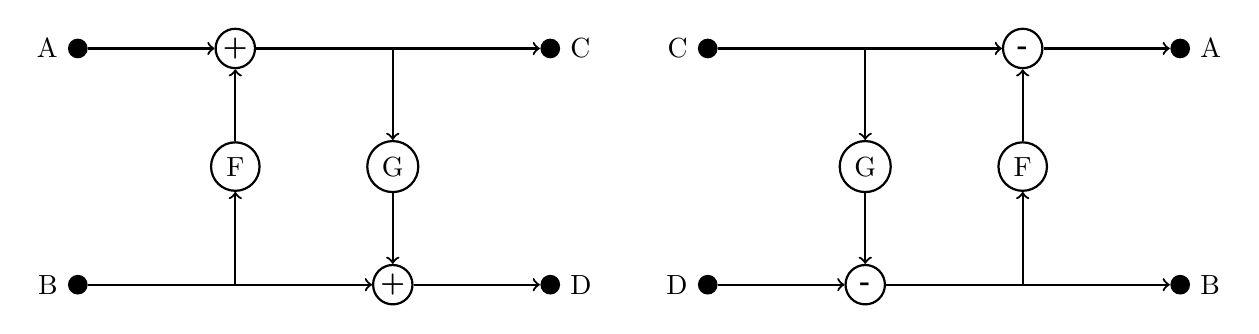
\begin{tikzpicture}[
                dot/.style = {circle, fill, inner sep = 0mm, minimum size = 2.5mm},
                op/.style = {draw, thick, circle, inner sep = 0mm, minimum size = 5mm},
                func/.style = {draw, thick, circle, inner sep = 1mm},
                arr/.style = {draw, thick, ->},
            ]
            \node (A) at (0, 3) [dot, label = left:A] {};
            \node (B) at (0, 0) [dot, label = left:B] {};
            \node (C) at (6, 3) [dot, label = right:C] {};
            \node (D) at (6, 0) [dot, label = right:D] {};

            \node (P1) at (2, 3) [op] {\textbf{+}};
            \node (P2) at (4, 0) [op] {\textbf{+}};

            \node (F) at (2, 1.5) [func] {F};
            \node (G) at (4, 1.5) [func] {G};

            \path[arr] (A) -- (P1);
            \path[arr] (P1) -- (C);
            \path[arr] (B) -- (P2);
            \path[arr] (P2) -- (D);
            \path[arr] (2, 0) -- (F);
            \path[arr] (F) -- (P1);
            \path[arr] (4, 3) -- (G);
            \path[arr] (G) -- (P2);

            \node (A) at (14, 3) [dot, label = right:A] {};
            \node (B) at (14, 0) [dot, label = right:B] {};
            \node (C) at (8, 3) [dot, label = left:C] {};
            \node (D) at (8, 0) [dot, label = left:D] {};

            \node (P1) at (12, 3) [op] {\textbf{-}};
            \node (P2) at (10, 0) [op] {\textbf{-}};

            \node (F) at (12, 1.5) [func] {F};
            \node (G) at (10, 1.5) [func] {G};

            \path[arr] (P1) -- (A);
            \path[arr] (C) -- (P1);
            \path[arr] (P2) -- (B);
            \path[arr] (D) -- (P2);

            \path[arr] (12, 0) -- (F);
            \path[arr] (10, 3) -- (G);
            \path[arr] (F) -- (P1);
            \path[arr] (G) -- (P2);
        \end{tikzpicture}
        \caption{Dataflow path of a lifting step and its derived inverse.\label{fig:lift}}
    \end{figure}

\subsection{Complex multiplication}
\begin{figure}
    \centering
    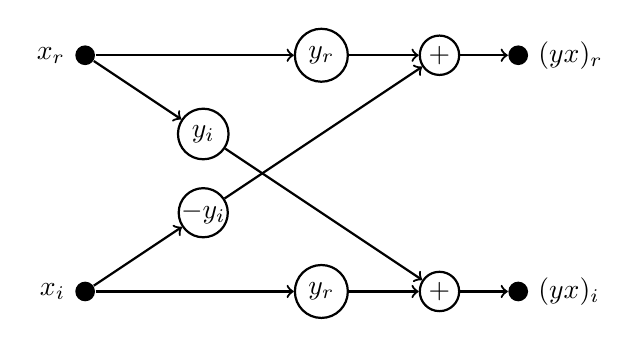
\begin{tikzpicture}[
            dot/.style = {circle, fill, inner sep = 0mm, minimum size = 2.5mm},
            op/.style = {draw, thick, circle, inner sep = 0mm, minimum size = 5mm},
            func/.style = {draw, thick, circle, inner sep = 1mm},
            arr/.style = {draw, thick, ->},
        ]
        \node (XR) [dot, label=left:$x_r$] at (0,3){};
        \node (XI) [dot, label=left:$x_i$] at (0,0){};
        \node (YXR) [dot, label=right:$(yx)_r$] at (5.5,3){};
        \node (YXI) [dot, label=right:$(yx)_i$] at (5.5,0){};

        \node (P1) [op] at (4.5, 3) {+};
        \node (P2) [op] at (4.5, 0) {+};
        \node (YR1) [func] at (3.0, 3) {$y_r$};
        \node (YR2) [func] at (3.0, 0) {$y_r$};

        \node (YI1) [func] at (1.5, 2) {$y_i$};
        \node (YI2) [op] at (1.5, 1) {$-y_i$};

        \path[arr] (XR) -- (YR1);
        \path[arr] (YR1) -- (P1);
        \path[arr] (P1) -- (YXR);

        \path[arr] (XI) -- (YR2);
        \path[arr] (YR2) -- (P2);
        \path[arr] (P2) -- (YXI);

        \path[arr] (XR) -- (YI1);
        \path[arr] (YI1) -- (P2);

        \path[arr] (XI) -- (YI2);
        \path[arr] (YI2) -- (P1);
    \end{tikzpicture}
    \caption{Dataflow path for complex multiplication.\label{fig:complexmula}}
\end{figure}

\begin{figure}
    \centering
    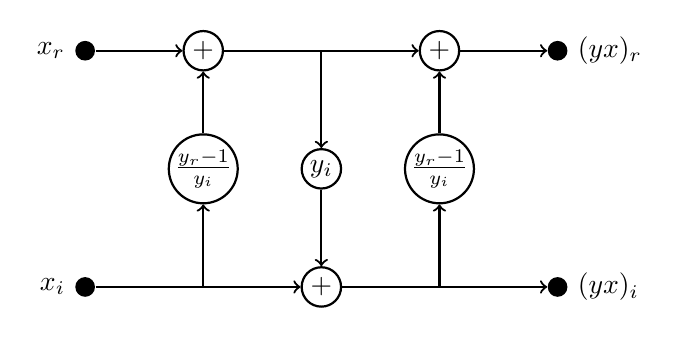
\begin{tikzpicture}[
            dot/.style = {circle, fill, inner sep = 0mm, minimum size = 2.5mm},
            op/.style = {draw, thick, circle, inner sep = 0mm, minimum size = 5mm},
            func/.style = {draw, thick, circle, inner sep = 1mm},
            arr/.style = {draw, thick, ->},
        ]
        \node (xr) [dot, label=left:$x_r$] at (0,3){};
        \node (xi) [dot, label=left:$x_i$] at (0,0){};
        \node (yxr) [dot, label=right:$(yx)_r$] at (6,3){};
        \node (yxi) [dot, label=right:$(yx)_i$] at (6,0){};

        \node (a) [op] at (1.5, 1.5) {$\frac{y_r - 1}{y_i}$};
        \node (b) [op] at (3, 1.5) {$y_i$};
        \node (c) [op] at (4.5, 1.5) {$\frac{y_r - 1}{y_i}$};

        \node (p1) [op] at (1.5, 3){+};
        \node (p2) [op] at (3, 0){+};
        \node (p3) [op] at (4.5, 3){+};

        \path[arr] (xr) -- (p1);
        \path[arr] (p1) -- (p3);
        \path[arr] (p3) -- (yxr);

        \path[arr] (xi) -- (p2);
        \path[arr] (p2) -- (yxi);

        \path[arr] (1.5, 0) -- (a);
        \path[arr] (a) -- (p1);

        \path[arr] (3, 3) -- (b);
        \path[arr] (b) -- (p2);

        \path[arr] (4.5, 0) -- (c);
        \path[arr] (c) -- (p3);
    \end{tikzpicture}
    \caption{Complex multiplication using lifting steps.\label{fig:complexmulb}}
\end{figure}

\subsection{Reversible convolution} % TODO: is 'convolution' the right word?
\begin{figure}
    \centering
    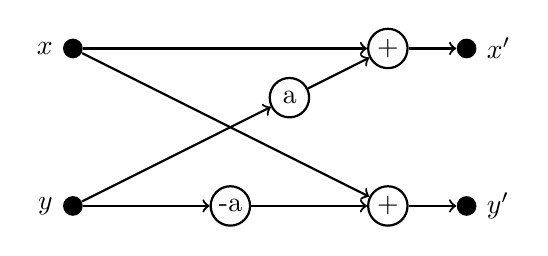
\begin{tikzpicture}[
            dot/.style = {circle, fill, inner sep = 0mm, minimum size = 2.5mm},
            op/.style = {draw, thick, circle, inner sep = 0mm, minimum size = 5mm},
            func/.style = {draw, thick, circle, inner sep = 1mm},
            arr/.style = {draw, thick, ->},
        ]
        \node (x) [dot, label=left:$x$] at (0,2){};
        \node (y) [dot, label=left:$y$] at (0,0){};
        \node (xp) [dot, label=right:$x'$] at (5,2){};
        \node (yp) [dot, label=right:$y'$] at (5,0){};

        \node (a1) [op] at (2.75, 1.375) {a};
        \node (a2) [op] at (2, 0) {-a};
        \node (p1) [op] at (4, 2) {+};
        \node (p2) [op] at (4, 0) {+};

        \path[arr] (x) -- (p1);
        \path[arr] (p1) -- (xp);
        \path[arr] (y) -- (a2);
        \path[arr] (a2) -- (p2);
        \path[arr] (p2) -- (yp);

        \path[arr] (x) -- (p2);

        \path[arr] (y) -- (a1);
        \path[arr] (a1) -- (p1);
    \end{tikzpicture}
    \caption{FFT convolution.\label{fig:conva}}
\end{figure}

\begin{figure}
    \centering
    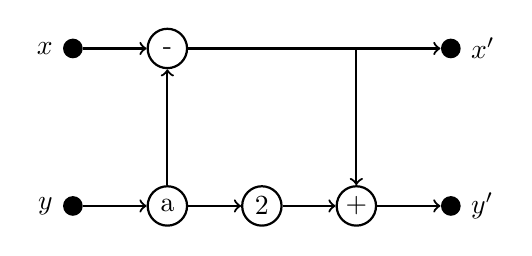
\begin{tikzpicture}[
            dot/.style = {circle, fill, inner sep = 0mm, minimum size = 2.5mm},
            op/.style = {draw, thick, circle, inner sep = 0mm, minimum size = 5mm},
            func/.style = {draw, thick, circle, inner sep = 1mm},
            arr/.style = {draw, thick, ->},
        ]
        \node (x) [dot, label=left:$x$] at (0,2){};
        \node (y) [dot, label=left:$y$] at (0,0){};
        \node (xp) [dot, label=right:$x'$] at (4.8,2){};
        \node (yp) [dot, label=right:$y'$] at (4.8,0){};

        \node (a) [op] at (1.2,0){a};
        \node (t) [op] at (2.4,0){2};
        \node (m) [op] at (1.2,2){-};
        \node (p) [op] at (3.6,0){+};

        \path[arr] (x) -- (m);
        \path[arr] (m) -- (xp);
        \path[arr] (y) -- (a);
        \path[arr] (a) -- (m);
        \path[arr] (a) -- (t);
        \path[arr] (t) -- (p);
        \path[arr] (p) -- (yp);
        \path[arr] (3.6,2) -- (p);
    \end{tikzpicture}
    \caption{Lifting steps for convolution.\label{fig:convb}}
\end{figure}

\begin{lstlisting}
procedure mul2
    if y = 0 then
        y += x
        x += y
        y -= x / 2
    fi y = 0
\end{lstlisting}

% TODO: Mention that the paper doesn't actually try to make directly reversible convolution

\begin{lstlisting}
x -= y
call mul2
y += x
x <=> y
\end{lstlisting}
